\chapter{Performance Test}

As with many network protocols designed to transfer data quickly and reliably, there needs to be performance analysis. The performance of MCDTP is measured by throughput and packet loss.

\section{Test Environment}

The test environment used to test MCDTPi used commodity servers rented from a cloud computing company called DigitalOcean. Two servers were rented, one deployed in New York, USA and the second deployed in Amsterdam, Netherlands---the distance was deliberate to test MCDTPi over WAN. The rented servers were configured with 4 CPUs, 8GB of RAM, 80GB SSD, and 5TB of transfer and run Ubuntu 16.04LTS. DigitalOcean does not disclose any server specifications beyond this. The servers were further configured with the cross-platform version of .NET Framework, .NET Core 1.0.3, in order to execute the tests for MCDTPi.

The Ethernet link of both servers places a constraint on the size of transmitted packets. This constraint is know as the Maximum Transmission Unit. The MTU for both servers was 1500 bytes. The largest a packet can be is 1500 bytes before it gets fragmented into smaller packets. Fragmentation is not handled by MCDTP so MCDTPi was compiled with a UDP packet size set to 1400 bytes.

\section{Testing}

There were four test configurations applied to MCDTPi. All configurations used a 1GB file as the data source. Since both servers had 8GB of main memory, for each test, MCDTPi was able to hold the entire file in memory. Thus disk I/O was not a factor in performance. The variable between each test was the number of channels MCDTPi used on each test---single-, dual-, quad-, and octa-channel configurations.

Since throughput and packet loss are used as performance measurements, only the Data Transmission phase of MCDTP is tested. This is to test the unreliability of MCDTP. By measuring unreliability, it gives insight as to how much work would need to be done to provide reliability.

\subsection{Test Results}

For the following tests, the server in New York played the role of client and the Amsterdam server played the role of server, which was arbitrarily decided since exact specifications on the servers are unknown and thus could not weigh in on this.

Figures \ref{fig:tr-ct} and \ref{fig:tr-st} show the throughput in bytes for single-, dual-, and quad-channel configurations for both client and server hosts, respectively. These results are discussed in section \ref{sec:anlys}.

Average throughput, max throughput, and packet loss statistics can be seen in Figures \ref{fig:tr-at}, \ref{fig:tr-mt}, and \ref{fig:tr-pl}, respectively. Average throughput values are: Server $\rightarrow$ Single-Channel: 1.146Mbps, Dual-Channel: 2.893MBps, Quad-Channel: 0.545Mbps, Octa-Channel: 0Mbps, and Client $\rightarrow$ Single-Channel: 1.018Mbps, Dual-Channel: 2.398MBps, Quad-Channel: 0.52Mbps, Octa-Channel: 0Mbps. Max throughput values are: Server $\rightarrow$ Single-Channel: 4.385Mbps, Dual-Channel: 6.998MBps, Quad-Channel: 12.065Mbps, Octa-Channel: 0Mbps, and Client $\rightarrow$ Single-Channel: 3.879Mbps, Dual-Channel: 5.934MBps, Quad-Channel: 11.755Mbps, Octa-Channel: 0Mbps. Packet loss values are: Single-Channel $\rightarrow$ 14.06\%, Dual-Channel $\rightarrow$ 19.64\%, Quad-Channel $\rightarrow$ 87.97\%, and Octa-Channel $\rightarrow$ 100.0\%. These results are discussed in section \ref{sec:anlys}.

\section{Analysis}\label{sec:anlys}

The expected behavior of MCDTPi is that as resources increase with more channels, throughput and packet loss improve. The test results show that this behavior is partly true going from single-channel to dual-channel. Throughput improved two fold while packet loss had marginal degradation. However, performance worsened in both measurement for quad- and octa-channel configurations. Octa-channel was omitted in Figures \ref{fig:tr-ct} and \ref{fig:tr-st} because tests stalled and yielded no data. Though the Figure \ref{fig:tr-mt} shows quad-channel achieving the highest throughput, it had an average throughput that was half that of the single-channel. Quad-channel over 6 times greater packet loss as well. This is all around worse.

This outcome seems counter intuitive to what is expected. Nonetheless, this can be explained. To start, the single-channel itself is severely under-perfomant compared to other protocols like RBUDP and Tsunami. Those protocols achieve 500 times as much throughput compared to MCDTP. The major difference between this project and those is the use of asynchronous technology. Asynchronous programming is helps MCDTPi be reactive. The TPL library is the underlying framework for this, which is very robust and provides assurances that there is synchrony amongst the asynchronous behavior \cite{Leijen2009}. This assurance adds overhead to the overall performance of the application, which, in certain scenarios involving large computations, is not often a problem. However, MCDTPi uses asynchronous programming to handle packets. All I/O operations are handled this way as well. These simple asynchronous tasks are numerous and are adding overhead to the overall performance.




\begin{figure}[ht]
\centering
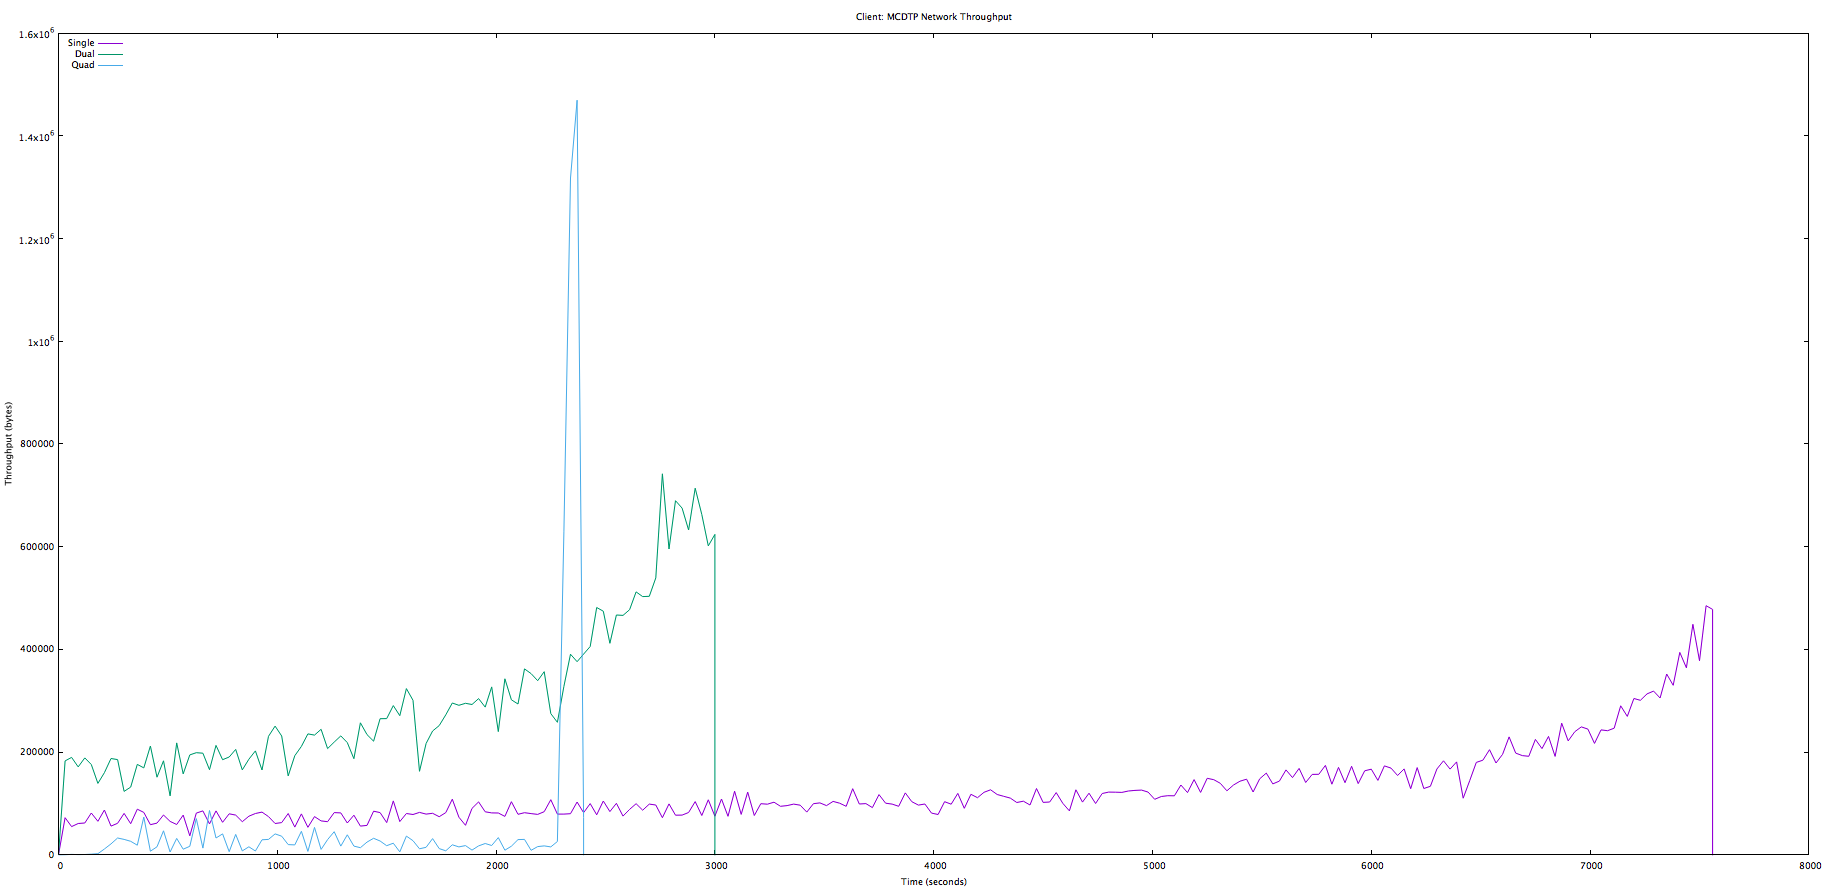
\includegraphics[scale=0.4]{TestResultClientThroughput}
\caption{Client Throughput}
\label{fig:tr-ct}
\end{figure}

\begin{figure}[ht]
\centering
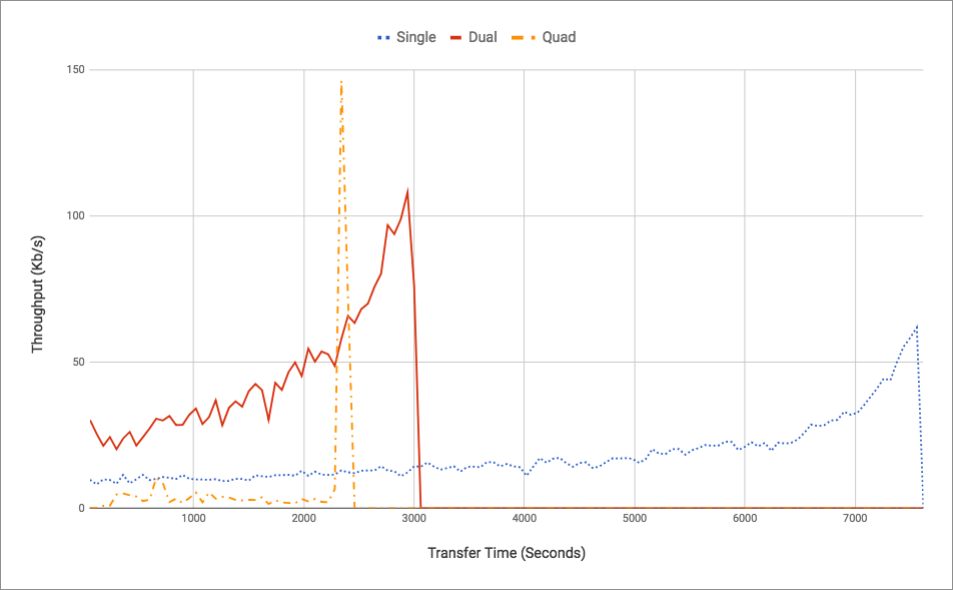
\includegraphics[scale=0.4]{TestResultServerThroughput}
\caption{Server Throughput}
\label{fig:tr-st}
\end{figure}

\begin{figure}[ht]
\centering
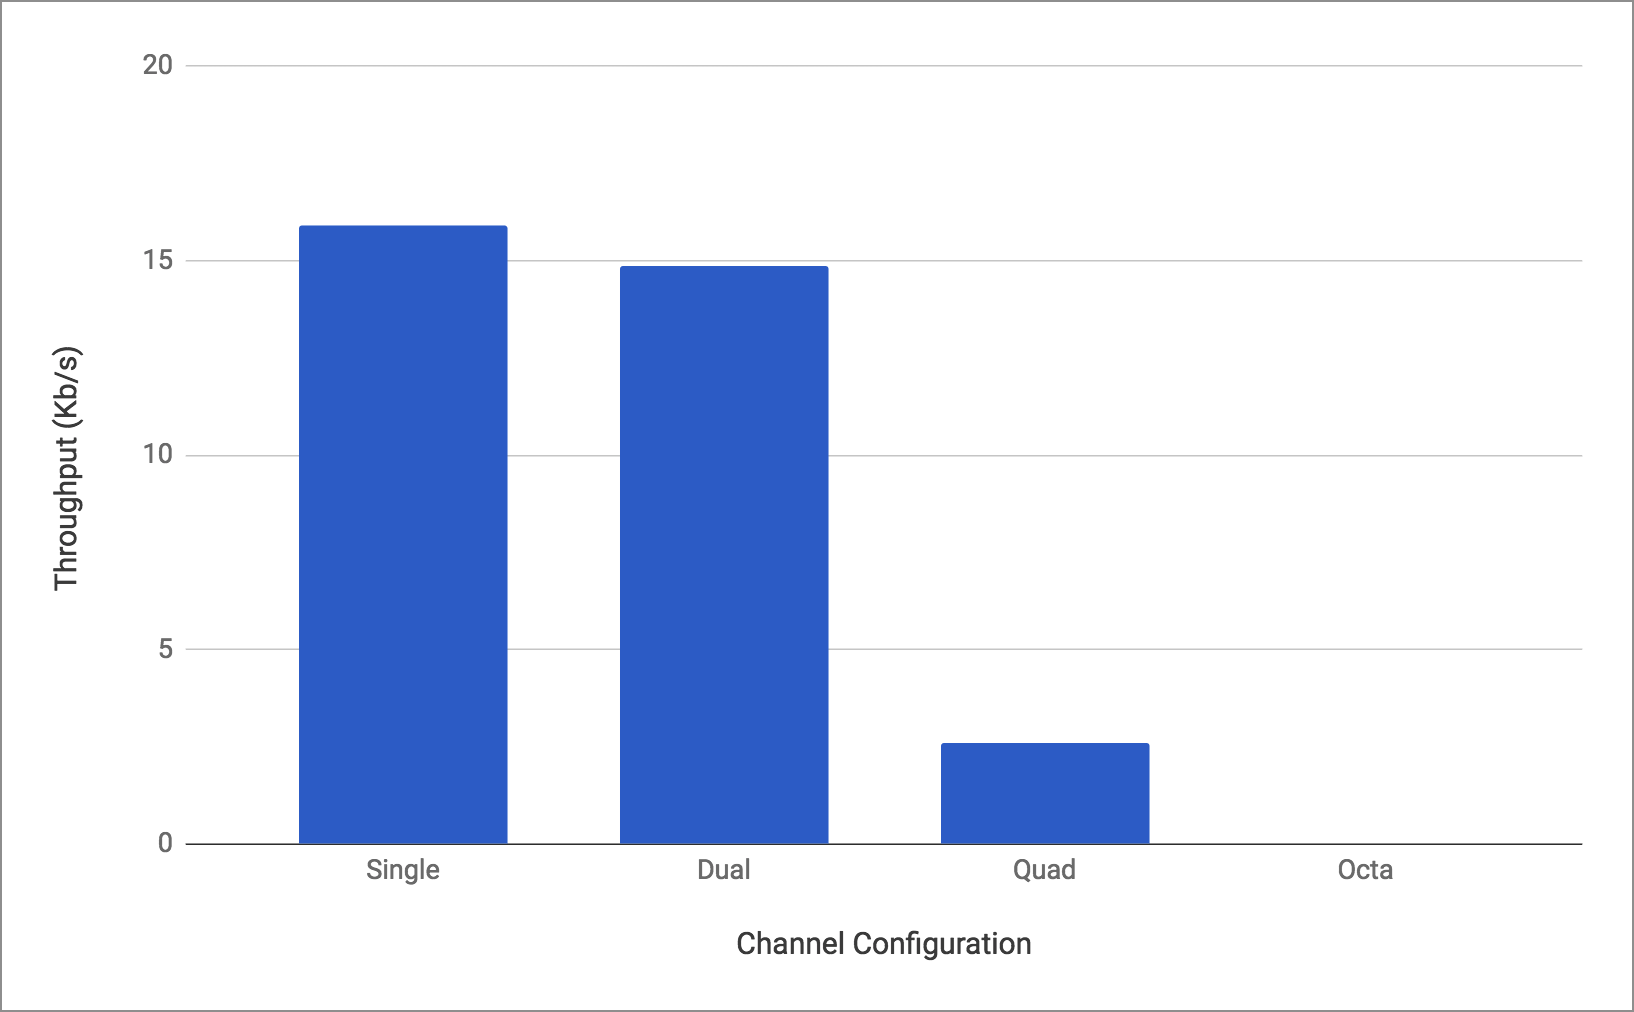
\includegraphics[scale=0.4]{TestResultAverageThroughput}
\caption{Average Throughput}
\label{fig:tr-at}
\end{figure}

\begin{figure}[ht]
\centering
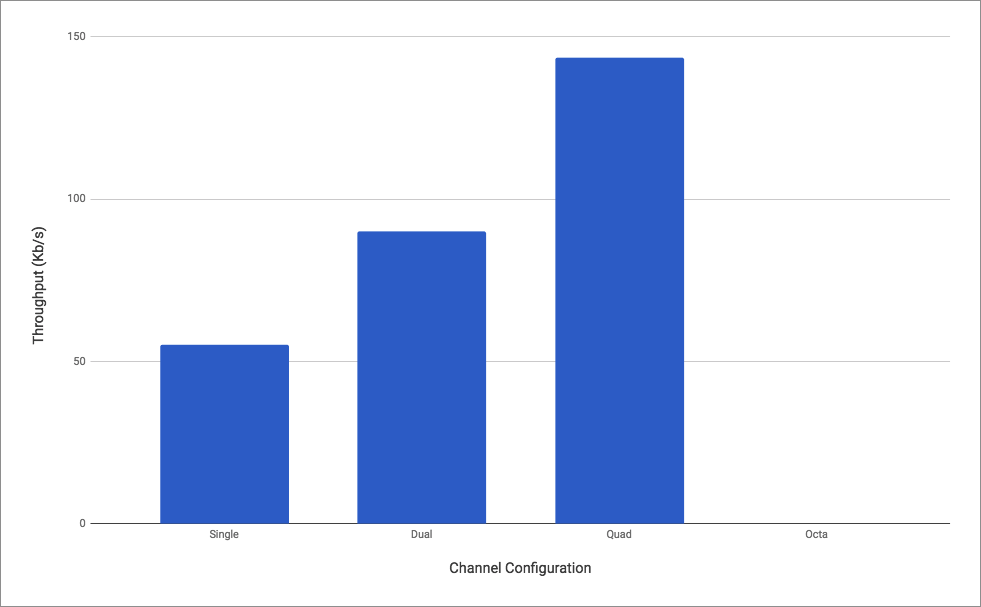
\includegraphics[scale=0.4]{TestResultMaxThroughput}
\caption{Max Throughput}
\label{fig:tr-mt}
\end{figure}

\begin{figure}[ht]
\centering
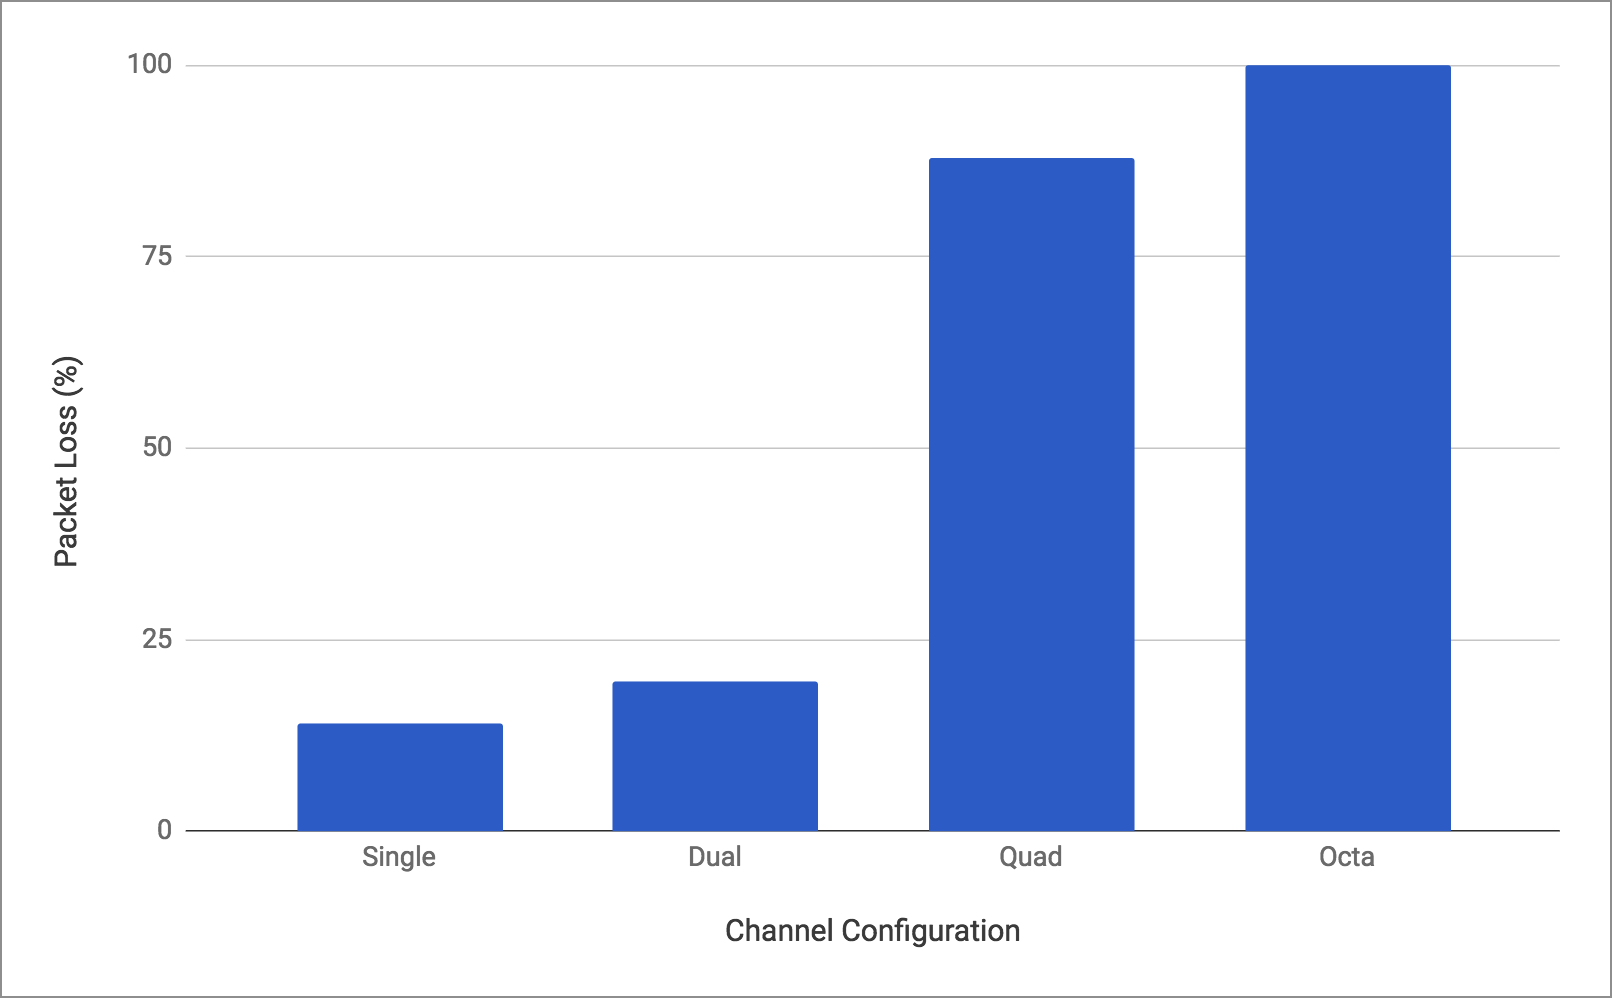
\includegraphics[scale=0.4]{TestResultPacketLoss}
\caption{Packet Loss}
\label{fig:tr-pl}
\end{figure}